\section{Vor dem Fest}
\subsection{Getränke und Equipment}
\begin{itemize}
  \item Auf Paletten an der zugeordneten Lieferzone:
    \begin{itemize}
      \item Bier- und Ciderfässer
      \item Non-Alk und Bier in Kästen
      \item Hard-Alk in Kartons (ab ca. 15:00 Uhr)
      \item Zapfanlagen
      \item Becher in Plastikkisten (\SI{0.3}{\litre} \& \SI{0.5}{\litre})
      \item Kühlschränke

        Bänder um die Kühlschränke \textbf{unbedingt} aufheben!
      \item Biertischgarnituren
      \item Eis in Gefriertruhen oder Thermoboxen
    \end{itemize}
  \item CO$_2$-Flaschen sind im Müllgang. Vorsichtig tragen! Mit Kabelbindern an Thekenelement festmachen und so gegen Umfallen schützen!
  \item Equipment abholen:
    \begin{itemize}
      \item Thekenkisten mit Klebeband, Zangen, Kabelbindern usw.\ sind im Lager (Raum A120)
      \item Helferkisten mit T-Shirts, Bändern usw.\ sind in der Helferzentrale, dieses Jahr in F107!
    \end{itemize}
  \item Pavillons sind bereits aufgebaut
  \item Feuerlöscher stehen bereit
\end{itemize}
% ---
\subsection{Thekenaufbau}
Siehe Abbildungen \ref{theke2d} und \ref{theke3d}.
\begin{figure}[h]
  \centering
  \begin{subfigure}[t]{0.45\textwidth}
    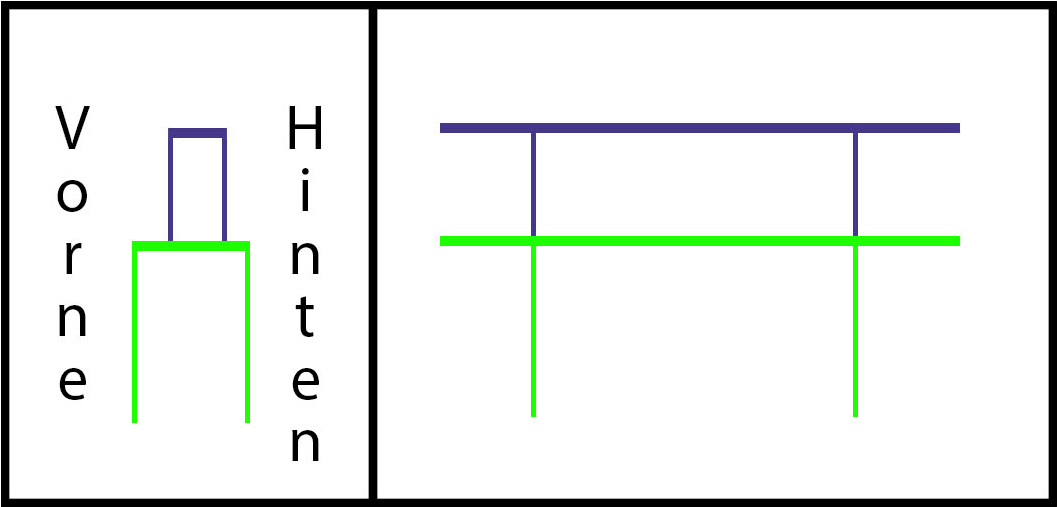
\includegraphics[width=\textwidth]{2d_1.png}
    \caption{Einen Tisch aufstellen und eine aufgeklappte Bank darauf stellen.}
  \end{subfigure}
  \hfill
  \begin{subfigure}[t]{0.45\textwidth}
    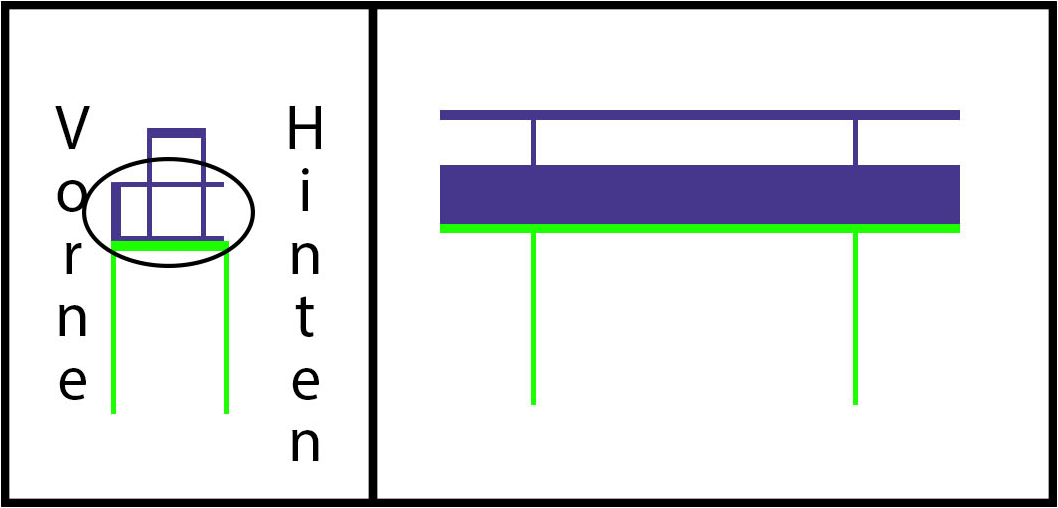
\includegraphics[width=\textwidth]{2d_2.png}
    \caption{Eine Bank aufklappen, aber die diagonalen Arretierungen eingeklappt lassen. Die Bank senkrecht zum Tisch hinlegen und alle drei Teile mit Kabelbindern befestigen, aber noch nicht ganz festzurren.}
  \end{subfigure}
  \centering
  \begin{subfigure}[t]{0.45\textwidth}
    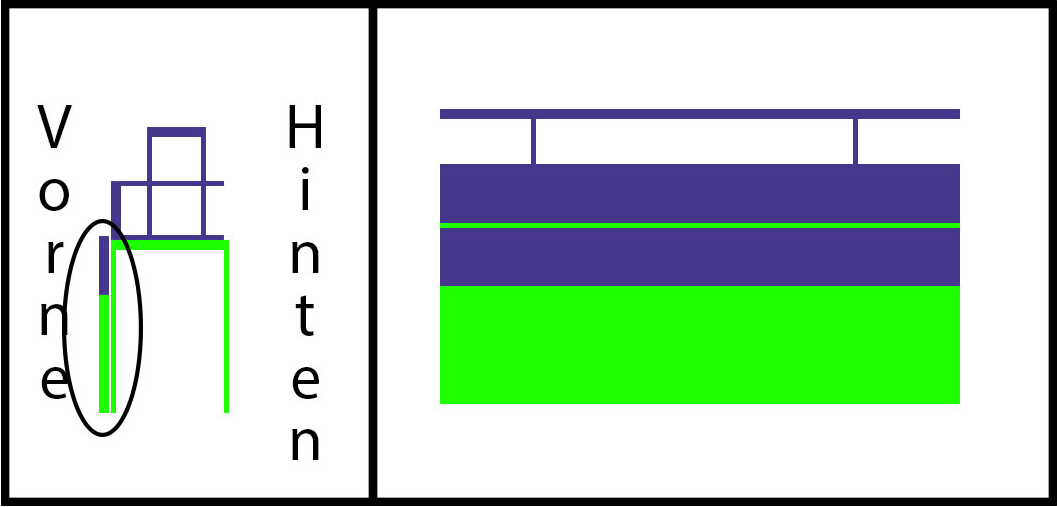
\includegraphics[width=\textwidth]{2d_3.png}
    \caption{Die Vorderseite mit 1 Tisch und 2 Bänken, oder 3 Bänken verkleiden und mit Kabelbindern verbinden (die Beine jeweils eingeklappt lassen, sonst stehen sie innen über).}
  \end{subfigure}
  \hfill
  \begin{subfigure}[t]{0.45\textwidth}
    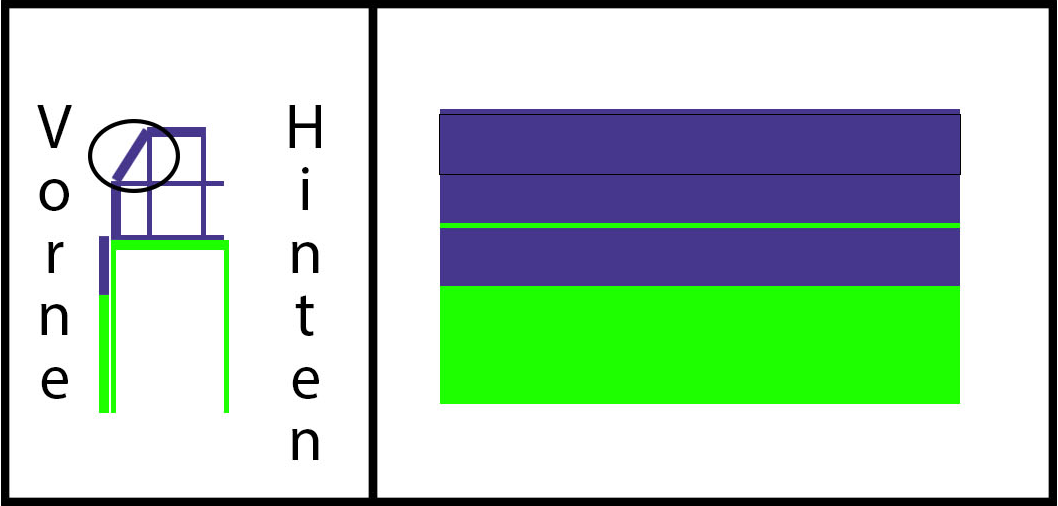
\includegraphics[width=\textwidth]{2d_4.png}
    \caption{Eine Bank (auch ohne Beine) schräg zwischen der liegenden und der stehenden Bank einspannen und mit Kabelbindern festzurren. Die Elemente untereinander anschließend mit Spanngurten/Kabelbindern verbinden.}
  \end{subfigure}
  \caption{Aufbau einer Theke aus 2 Tischen (grün) und 4 Bänken (blau) oder 1 Tisch und 6 Bänken.}
  \label{theke2d}
\end{figure}

\begin{figure}[htp]
  \begin{subfigure}[t]{0.45\textwidth}
    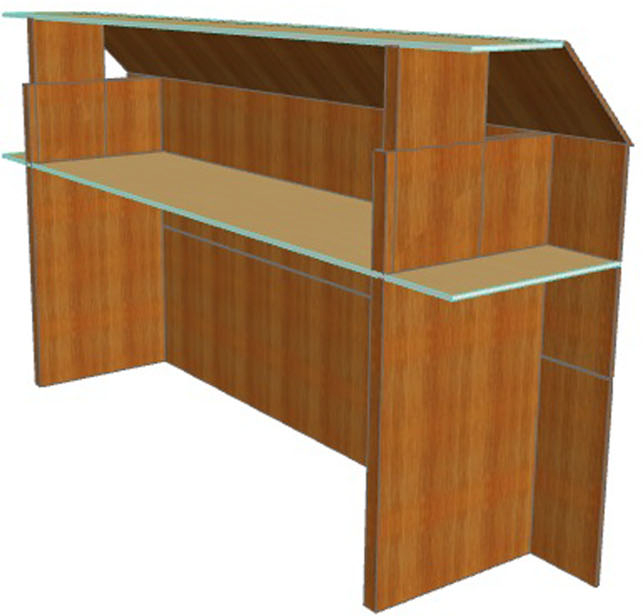
\includegraphics[width=\textwidth]{3d_hinten.png}
    \caption{Ansicht von hinten.}
  \end{subfigure}
  \begin{subfigure}[t]{0.45\textwidth}
    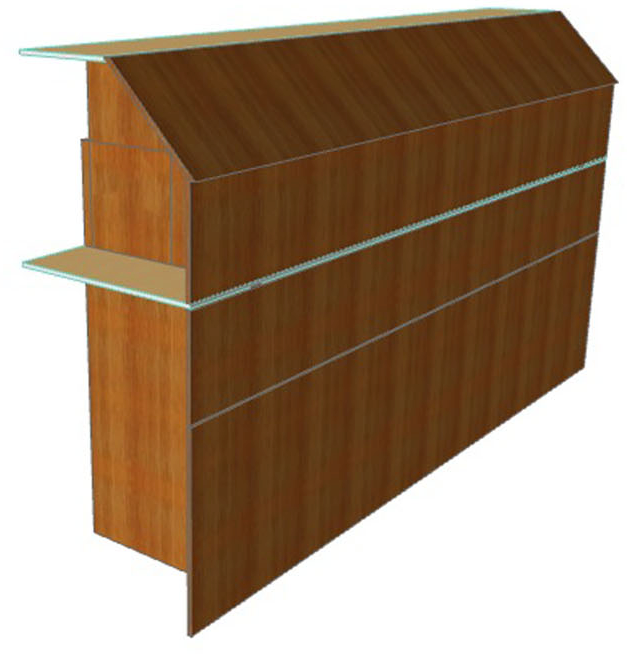
\includegraphics[width=\textwidth]{3d_vorne.png}
    \caption{Ansicht von vorne.}
  \end{subfigure}
  \caption{So sollte eure Theke mehr oder weniger aussehen.}
  \label{theke3d}
\end{figure}
% ---
\FloatBarrier
\subsection{Molton}
Ihr bekommt Molton -- schwarzen, schweren Stoff -- in Kisten von uns, mit dem ihr eure Theken verkleidet. Dafür nehmt ihr Stücke, die \SI{1.2}{\meter} oder \SI{1.3}{\meter} breit sind, also so hoch wie ein Thekenelement. Diese Stücke werden mit Klebeband am oberen Teil der schrängen Bank befestigt, sodass die gesamte Thekenfront verkleidet ist.\\
Der Molton ist wie alles andere vorkommissioniert.\\
\textbf{Muss bis 16:30 erledigt sein.}
% ---
\subsection{Schilder}
\begin{itemize}
  \item Geklebt werden darf auf \textbf{nur} auf unsere Aufbauten und Kühlschränke
  \item Alles nur mit Kreppband kleben und \textbf{niemals} auf verputzte oder gestrichene Wände!
  \item Aufgehängt werden müssen
    \begin{itemize}
      \item Thekenbeschilderung: Getränkeangebot, laminiert A4/A3 auf die Thekenelemente
      \item Jugendschutzgesetze
    \end{itemize}
  \item Eigene Banner der Fachschaft o.ä.\ müssen mit uns \textbf{rechtzeitig} vorher abgesprochen werden und brauchen in jedem Fall ein Brandschutzzertifikats (B1).

    Ohne Absprache mitgebrachte Sachen (Banner, Plakate etc.) können \textbf{nicht} aufgehängt werden!

    Bitte bringt auch keine Flyer oder Aufkleber eurer Fachschaft mit.
\end{itemize}
% ---
\subsection{Deadlines}
\begin{itemize}
  \item Zapfanlagen fertig bis \textbf{16:30} für Getränkerundgang und Abnahme der Schankanlagen
  \item Thekenfronten fertig bis \textbf{16:30} für KVR-Rundgang um \textbf{17:00}
  \item Theke innen fertig aufbauen und betriebsfertig machen!

    Alle Getränke zählen und in die angehängte Liste (\emph{Vorher}) eintragen. Einer der Getränkeorgas (Felix, Markus oder Christoph) holt sie dann vor dem Fest ab.
  \item \Large{Fest beginnt um \textbf{19:00}!}
\end{itemize}
\FloatBarrier
